\documentclass[tikz,border=5pt]{standalone}
\usepackage{tikz}
\usetikzlibrary{positioning,fit,backgrounds,calc,shapes.geometric}
\usepackage{graphicx}
\usepackage{xcolor}

\definecolor{gitopsblue}{RGB}{51,108,229}
\definecolor{manualgray}{RGB}{102,102,102}
\definecolor{driftred}{RGB}{229,115,115}
\definecolor{warnorange}{RGB}{255,167,38}
\definecolor{okgreen}{RGB}{76,175,80}

\begin{document}
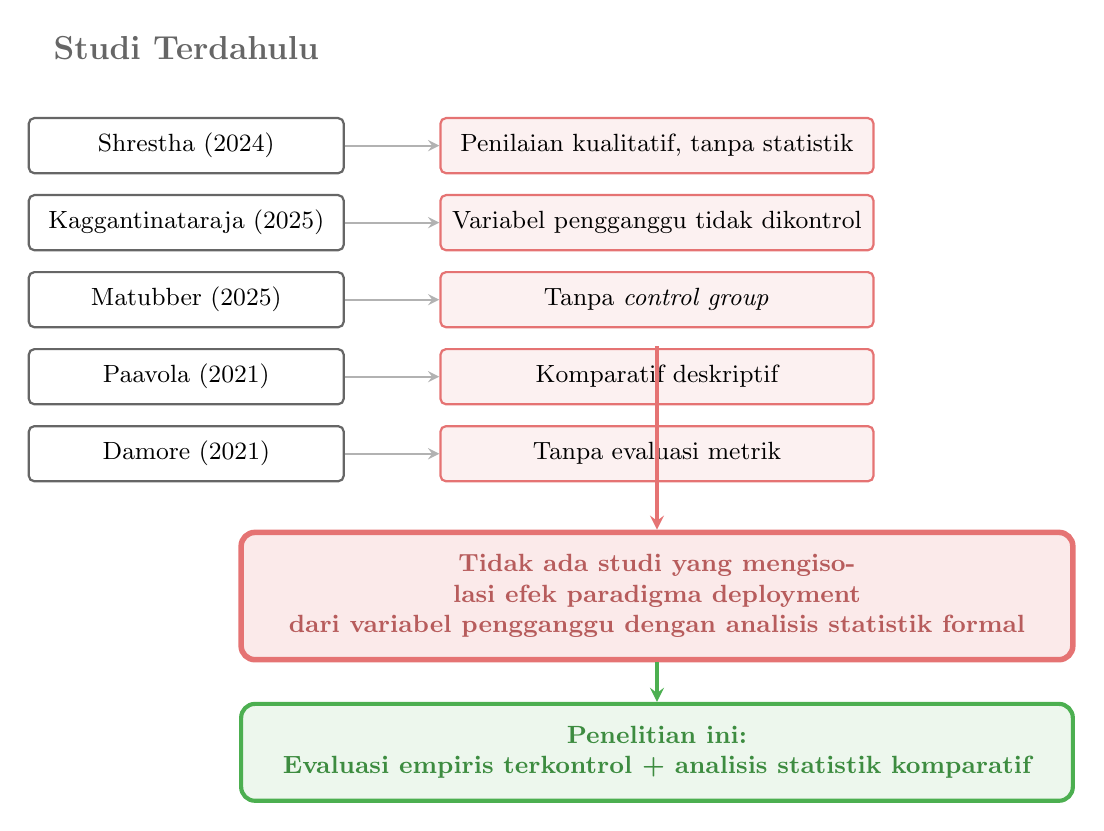
\begin{tikzpicture}[
    node distance=0.35cm,
    study/.style={rectangle, rounded corners=2pt, draw=manualgray, fill=white,
                  minimum width=4.0cm, minimum height=0.7cm, align=center,
                  line width=0.8pt, font=\small},
    limitation/.style={rectangle, rounded corners=2pt, draw=driftred, fill=driftred!10,
                      minimum width=5.5cm, minimum height=0.7cm, align=center,
                      line width=0.8pt, font=\small},
    gapbox/.style={rectangle, rounded corners=5pt, draw=driftred, fill=driftred!15,
                   inner sep=8pt, line width=2pt},
    arrow/.style={->, >=stealth, line width=0.8pt, draw=manualgray!50}
]

% Title
\node[font=\large\bfseries, text=manualgray] (title) {Studi Terdahulu};

% Studies
\node[study, below=0.6cm of title] (s1) {Shrestha (2024)};
\node[study, below=0.25cm of s1] (s2) {Kaggantinataraja (2025)};
\node[study, below=0.25cm of s2] (s3) {Matubber (2025)};
\node[study, below=0.25cm of s3] (s4) {Paavola (2021)};
\node[study, below=0.25cm of s4] (s5) {Damore (2021)};

% Limitations
\node[limitation, right=1.2cm of s1] (l1) {Penilaian kualitatif, tanpa statistik};
\node[limitation, right=1.2cm of s2] (l2) {Variabel pengganggu tidak dikontrol};
\node[limitation, right=1.2cm of s3] (l3) {Tanpa \textit{control group}};
\node[limitation, right=1.2cm of s4] (l4) {Komparatif deskriptif};
\node[limitation, right=1.2cm of s5] (l5) {Tanpa evaluasi metrik};

% Arrows
\draw[arrow] (s1) -- (l1);
\draw[arrow] (s2) -- (l2);
\draw[arrow] (s3) -- (l3);
\draw[arrow] (s4) -- (l4);
\draw[arrow] (s5) -- (l5);

% Gap message
\node[gapbox, below=0.6cm of l5, text width=10cm, align=center, font=\small\bfseries, text=driftred!80!black] (gap) {
    Tidak ada studi yang mengisolasi efek paradigma deployment\\
    dari variabel pengganggu dengan analisis statistik formal
};

% Arrow from all limitations to gap
\draw[->, >=stealth, line width=1.2pt, draw=driftred] ($(l3)!0.5!(l4) + (0,-0.1)$) -- (gap);

% Our contribution
\node[rectangle, rounded corners=5pt, draw=okgreen, fill=okgreen!10,
      inner sep=8pt, line width=1.5pt, below=0.5cm of gap, 
      text width=10cm, align=center, font=\small\bfseries, text=okgreen!80!black] (ours) {
    Penelitian ini:\\
    Evaluasi empiris terkontrol + analisis statistik komparatif
};

\draw[->, >=stealth, line width=1.2pt, draw=okgreen] (gap) -- (ours);

\end{tikzpicture}
\end{document}